\section{Implementation} \label{sec:implementation}
This section will discuss the implementation of each module and the way they integrate together to make the computer. Figure \ref{fig:computer} shows the computer as it was in January 25, which was its first working state. In Figure \ref{fig:computer_parts} the overlays show where each of the modules are located.

\begin{figure}[H]
  \centering
  % TODO: high resulotion version
  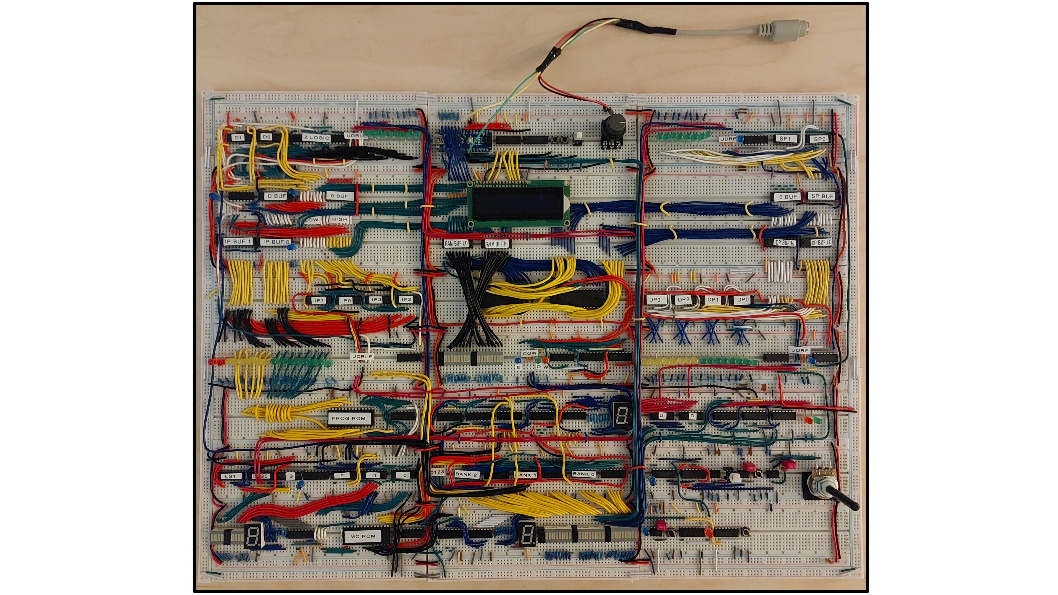
\includegraphics[width=0.9\textwidth]{img/computer}
  \caption{Prototype in January 2025.}
  \label{fig:computer}
\end{figure}

\begin{figure}[H]
  \centering
  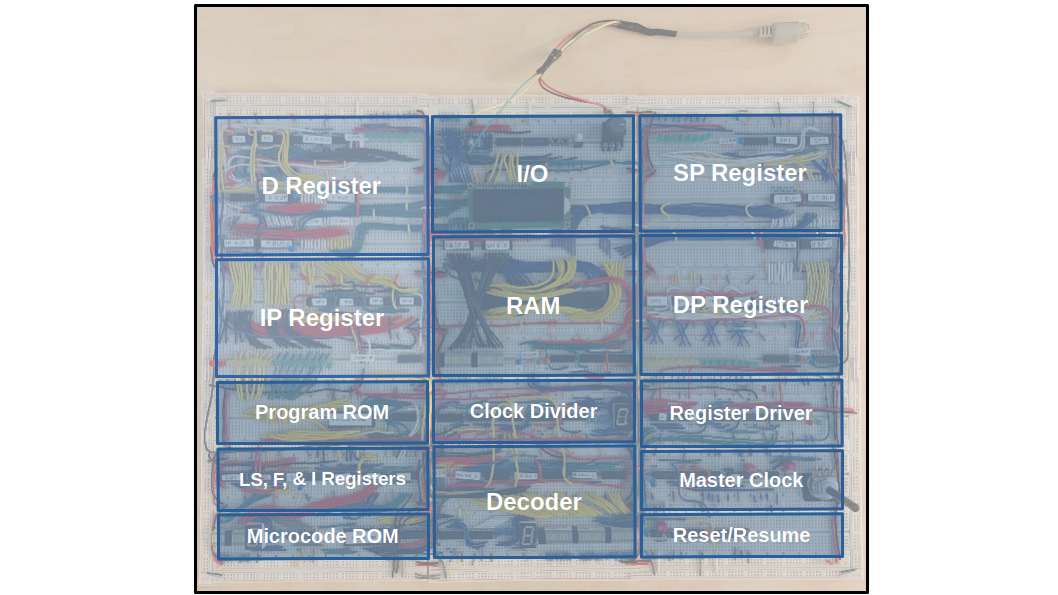
\includegraphics[width=0.9\textwidth]{img/computer_parts}
  \caption{Overview of the different parts of the computer.}
  \label{fig:computer_parts}
\end{figure}

%%%%%%% CLOCK

\subsection{Master Clock and Reset/Resume} \label{sec:clock}
\begin{figure}[H]
  \centering
  
\includegraphics[width=0.6\textwidth]{img/placeholder}
  \caption{Close up of the Master Clock and Reset/Resume Modules.}
  \label{fig:masterclockcloseup}
\end{figure}

The Master Clock module (MC) is located at the bottom right of the computer and is responsible for providing a heartbeat to most of the modules. The design of the clock is taken directly from Ben Eater's 8-bit computer video's \cite{beneater}. The automatic clock is generated by a 555 timer in astable mode. A 1M linear potentiometer is used together with a 1$\mu$ capacictor to control the frequency. Two additional 555 timers are used to debounce both the pushbutton for the manual clock and the latching push button which acts as a select between the two modes, as per Ben's design. 

The reason this module is called \emph{Master} Clock (rather than just Clock) is that the output of this module is not serving directly as the clock to all of the modules. For reasons becoming apparent when the implementation of the decoding process is discussed (see \ref{sec:implementation:clockdivider}), this clock is divided into 4 subclock-pulses, the last of which is sent to the modules. Effectively,  the frequency at which the computer operates is only one fourth that of the output from the MC.

The Reset/Resume module is directly underneath the clock and contains some logic to be able to reset the computer (necessary after applying power) and resuming the clock when it is halted. The HLT signal coming from the decoder is latched into a register (74LS173) from which the corresponding output bit is connected to the HLT input of the Master Clock selection logic. When the system is reset using the reset button or when the resume button is pressed, the HLT bit is cleared and the clock resumes. This allows for pausing and resuming the computer, effectively adding breakpoints in the code. The reset button itself is debounced in the same way as the manual clock button to ensure a stable transition. 

\subsubsection*{Stability}
When the output of the clock was first connected a counting register within the clock divider, it turned out that its output signal was too noisy for reliable operation of the counter. This register (74LS161) is sensitive to even very short pulses and the logic responsible for selecting either the automatic clock or the manual pulses was adding too much noise. The selection logic was modified to use a Schmitt Trigger (74LS14) at its output (rather than a regular inverter like the 74LS04) to improve output signal quality. A Schmitt Trigger acts as an inverter with different thresholds for each direction of inversion. This means it will invert any incoming signal above some voltage threshold but when the input goes below that same threshold shortly after due to noise, it will not change its output again until the signal drops significantly. Once the Schmitt Trigger was implemented, all stability issues went away.

\subsubsection*{Frequency Control}
The frequency of the waveform at the output of a 555 timer can be calculated using the formula from the datasheet \cite{datasheet:555}:
\begin{align}
  f=\frac{\ln{0.5}}{\left(R_A + 2R_B\right)C}
\end{align}
The value of $R_B$ is controlled by a potentiometer (up to $1M\Omega$) for fine control of the frequency. Assuming that the potentiometer has negligible resistance at its lowest setting, the maximum frequency is then determined by the values of $R_A$ and $C$, which can be set using 4 DIP switches to determine a frequency multiplier $M_f$:

\begin{align}
  f_{max} &\approx 1.44 \times M_F,\qquad \mathrm{where} \\
  M_f &= \frac{1}{R_AC} \label{eq:mf}
\end{align}

Two of these switches are connected to resistors of $100\Omega$ and $1k\Omega$, where the other two are connected to capacitors of $1\mu F$ and $0.1\mu F$. Table \ref{tab:fmultipliers} shows values of the multiplier for different combinations of selectable $R_A$ and $C$ values in our implementation. Given that the maximum multiplier is of the order $10^5$, frequencies in the order of 100 kHz can be achieved using this setting. Even higher frequencies, using even smaller capacitance or resistor values soon become unstable. See also section \ref{sec:performance} for more on performance benchmarks.

\begin{table}[H]
  \centering
  \setlength\extrarowheight{5pt}
  \begin{tabular}{cc|cc}
    \multicolumn{2}{c|}{\multirow{2}{*}{$M_f$}} & \multicolumn{2}{c}{$R_A(\Omega)$} \\
                            &          &  $10^2$  & $10^3$ \\ \hline
    \multirow{2}{*}{$C(F)$} & $10^{-6}$ &  $10^4$  & $10^3$ \\
                            & $10^{-7}$ &  $10^5$  & $10^4$ \\
  \end{tabular}
  \caption{Frequency multipliers for different combinations of $R_A$ and $C$.}
  \label{tab:fmultipliers}
\end{table}



\subsubsection*{Parts}
\begin{multicols}{2}
\begin{itemize}\itemsep0em
\item 4x NE555P (555 Timer)
\item 1x 74LS14 (Schmitt Trigger Inverter)
\item 1x 74LS00 (NAND)
\item 1x 74LS173 (4 bit register)
\item 1x 74LS32 (OR)
\item 4x $0.01\mu F$ ceramic capacitor
\item 1x $0.1\mu F$ ceramic capacitor
\item 3x $1\mu F$ capacitor
\item 3x tactile switch
\item 1x latching push button
\item 1x potentiometer (0-1M)
\item 6x 1K resistor
\item 1x 100$\Omega$ resistor
\item 1x 200K resistor
\item 1x 470K resistor
\item 1x Quad DIP switch
\end{itemize}
\end{multicols}

\subsubsection*{Schematic}
A full schematic is provided on the next page.
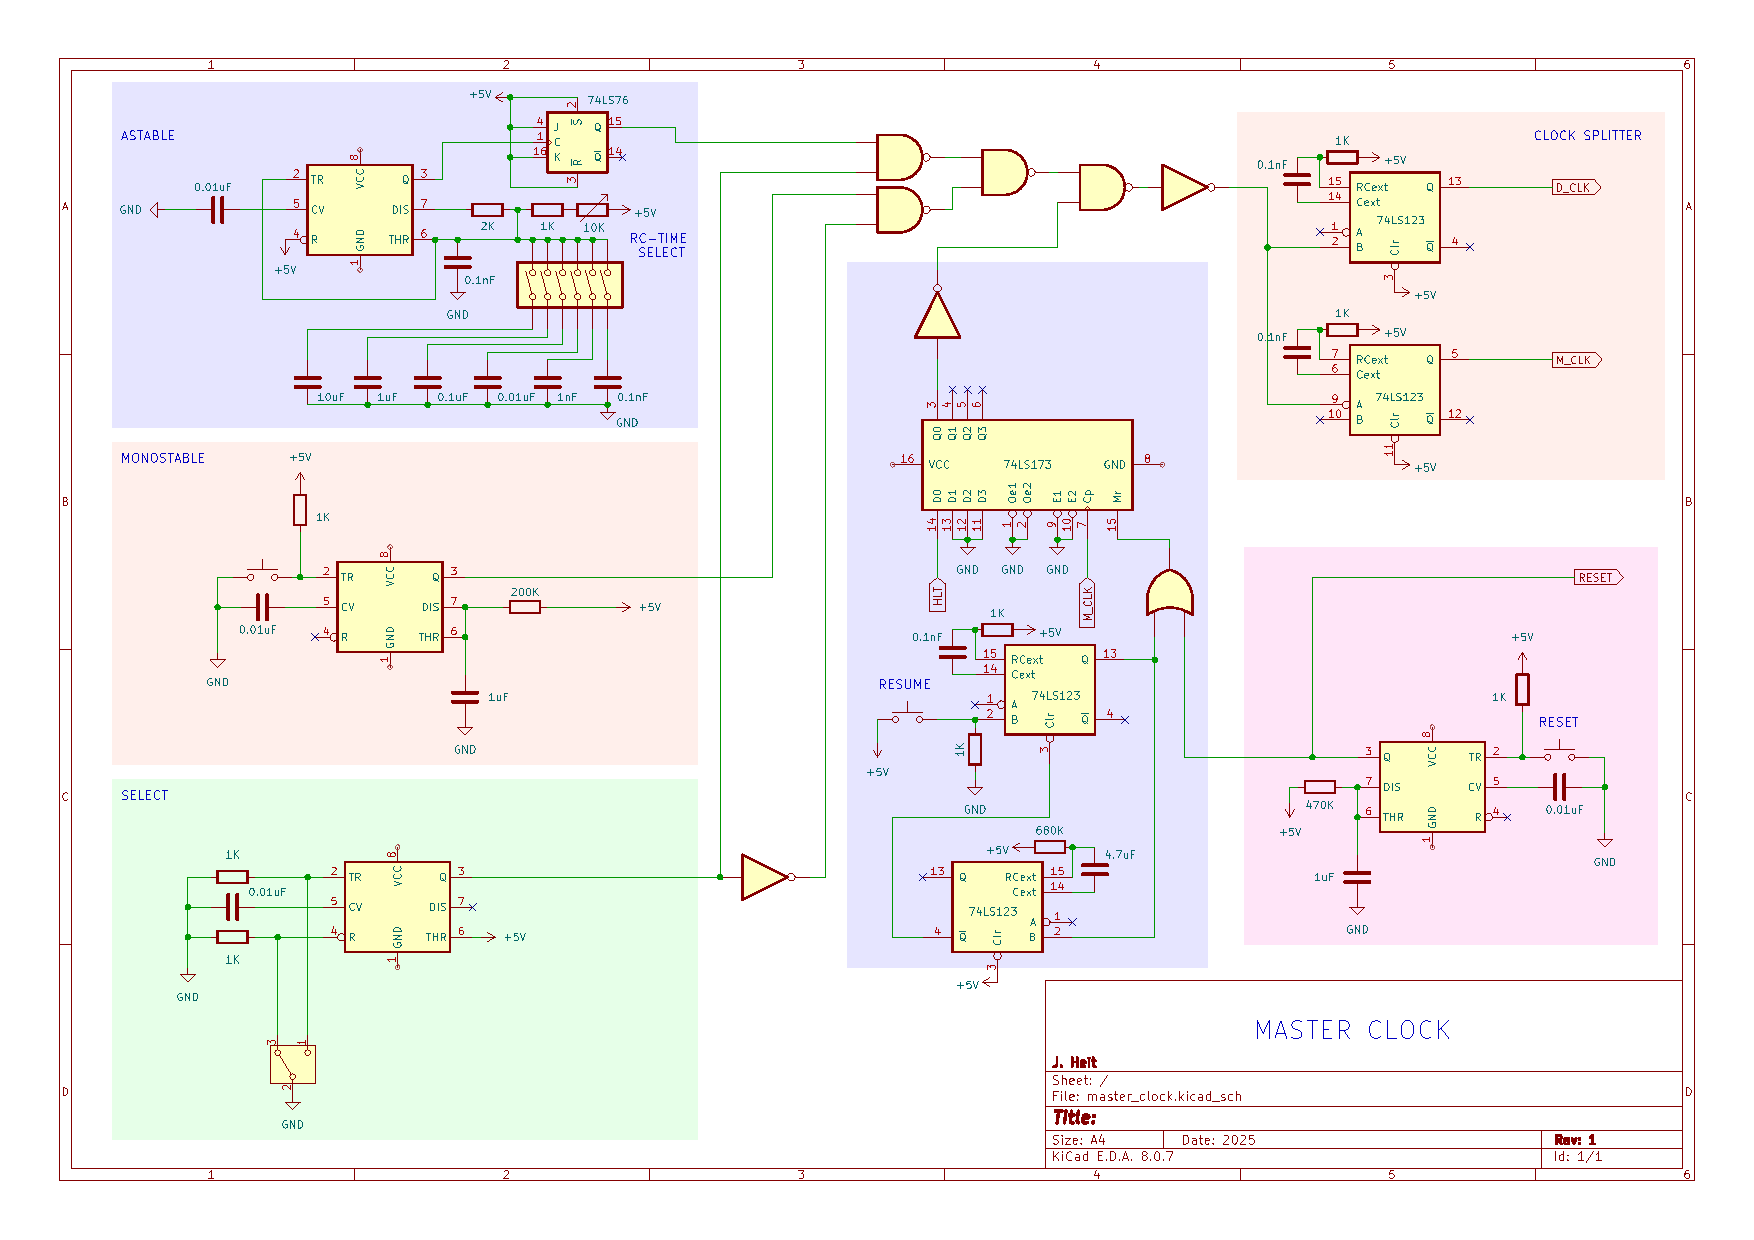
\includepdf[landscape=true]{schematics/masterclock.pdf}

%%%%%%% REGISTER DRIVER

\subsection{Register Driver} \label{sec:implementation:registerdriver}
\begin{figure}[H]
  % TODO: add annotations to the image
  \centering
  
\includegraphics[width=0.6\textwidth]{img/placeholder}
  \caption{Close up of the Register Driver Module.}
  \label{fig:registerdrivercloseup}
\end{figure}
The register driver is responsible for sending the correct signals to the counting input of the D, DP, SP, IP and LS registers. All of these are based around the 74LS193, which has a U and D input and requires one of them to be pulsed low in order to execute the corresponding action. For example, to decrement this register, a low pulse must be sent to the D input while U is kept high. As explained in section \ref{sec:architecture:controlunit}, we used a centralized driver to limit the number of logic IC's necessary to drive the registers and the total number of control signals necessary.

To limit the number of IC's, we chose to use NAND-gates instead of inverters and AND-gates. The truth table for this logic is shown in Table \ref{tab:registerdrivertruth}.

\begin{table}[h]
  \centering
  \begin{tabular}{ccc|cc|l}
    INC & DEC & CLC & U & D & Effect \\ \hline
    0   & 0   & 0   & 1 & 1 & - \\
    0   & 0   & 1   & 1 & 1 & - \\
    0   & 1   & 0   & 1 & 1 & - \\
    0   & 1   & 1   & 1 & 0 & Low pulse on D: decrement active register. \\
    1   & 0   & 0   & 1 & 1 & - \\
    1   & 0   & 1   & 0 & 1 & Low pulse on U: increment active register \\
    1   & 1   & 0   & 1 & 1 & - \\
    1   & 1   & 1   & 1 & 1 & - \\
  \end{tabular}
  \caption{Truth table for the register driver logic in order to comply with the 74LS193 counting registers.}
  \label{tab:registerdrivertruth}
\end{table}

The Register Driver takes 3 select-bits (control signals coming from the decoder) together with an INC and DEC signal and the clock (not the MC). The logic as seen in the schematic on the following page is responsible for providing the U and D inputs to the 74LS193 counters, each of which are sent to a demultiplexer (74LS138). The aforementioned register select signals are used to index these chips and address the appropriate registers (see also Table \ref{tab:registers}).

\subsubsection*{Parts}
\begin{itemize}\itemsep0em
\item 2x 74LS00 (NAND)
\item 1x 74LS86 (XOR)
\item 2x 74LS138 (3-to-8 demultiplexer)
\end{itemize}

\subsubsection*{Schematic}
A full schematic is provided on the next page.
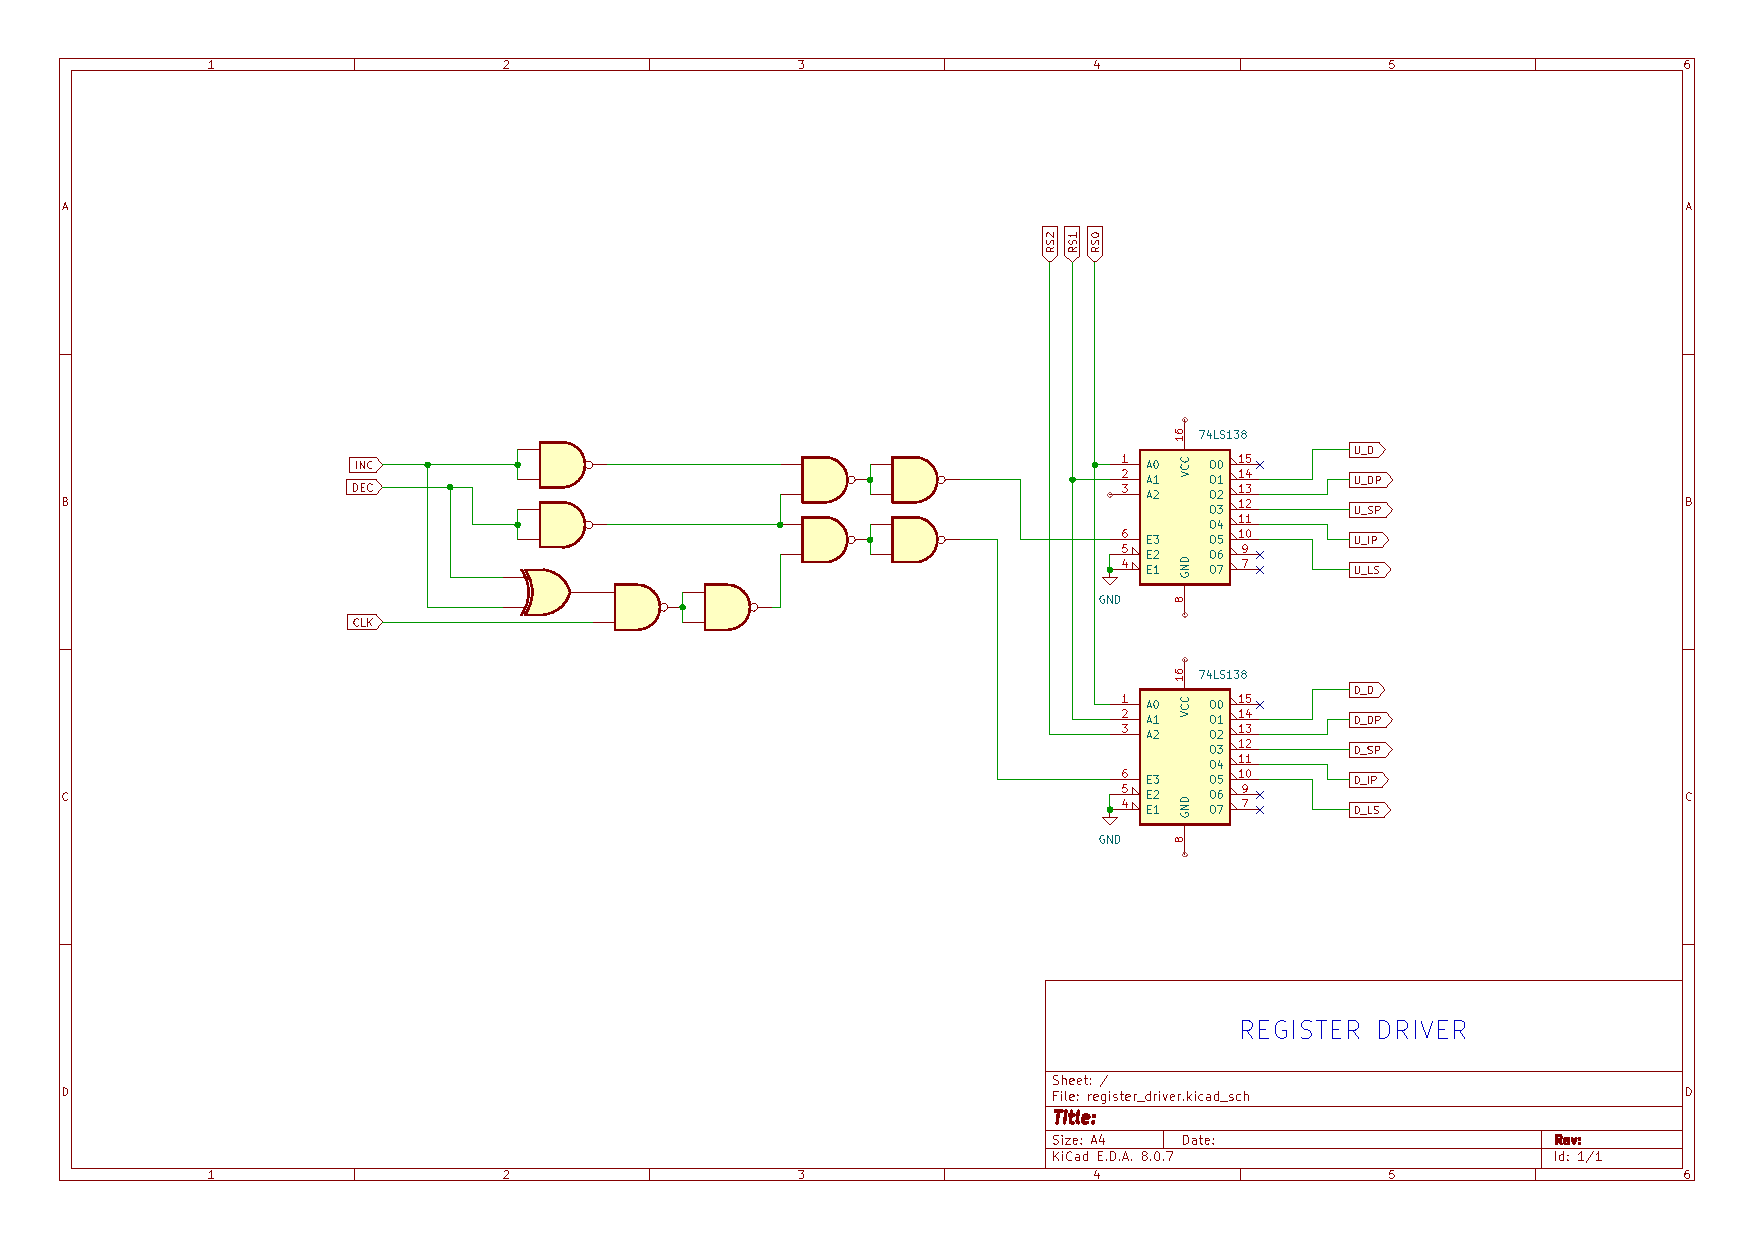
\includepdf[landscape=true]{schematics/registerdriver.pdf}

%%%%%%% DATA POINTER REGISTER

\subsection{DP Register Module}
\begin{figure}[H]
  \centering
  
\includegraphics[width=0.6\textwidth]{img/placeholder}
  \caption{Close up of the Data Pointer Register Module.}
  \label{fig:dpregcloseup}
\end{figure}

The datapointer register contains the address of the cell currently being operated on. It is a 16 bit value kept in four 74LS193 IC's because of the requirement that is should be able to be incremented and decremented. Their outputs are connected to the address bus through a pair of tristate buffers to prevent bus contention with the stack pointer. Because the first 256 bytes are reserved as the stack (where instruction pointer values can be stored to implement loops), the reset value of this register should be set to 0x0100. This is achieved by resetting all IC's except for the one containing the 3rd nibble, which is reset to one by hardcoding 0x1 to its inputs and connecting the reset line (through an inverter) to the load-pin instead.

This register is special in the sense that it is the only register that should be able to be reset at runtime seperately from all the other modules (through the DPR signal). This allowes it to be reset to its starting value after initializing the computer when power is first applied (see also Sections \ref{sec:sequences:init} and \ref{sec:sequences:home}). The RESET signal is therefor fed into an OR gate together with the DPR signal before going to the reset pins of the IC's.

Perhaps somewhat confusingly, the schematic (see next page) shows that the SP\_EN signal is used to enable the buffers. Since the bus is shared only between the stack pointer and data pointer, the same signal can be used to enable and disable their respective buffers: when the stack pointer is enabled, the data pointer should be disabled and vice versa. Since the output enable pin of the 74LS245 is active low, the SP\_EN can be fed directly into it. On the side of the stack pointer, the same signal goes through an inverter before going into the buffer. By default, when the stack pointer is not enabled, the datapointer will provide the address to the RAM. The RAM address input lines will never be floating which means that the contents of the current memory cell (in RAM) will always be visible in the computer.

\subsubsection*{Parts}
\begin{itemize}\itemsep0em
\item 1x 74LS04 (NOT)
\item 1x 74LS32 (OR)
\item 4x 74LS193 (Up/Down Counting Register)
\item 2x 74LS245 (Tristate Buffer)
\end{itemize}


\subsubsection*{Schematic}
A full schematic is provided on the next page.
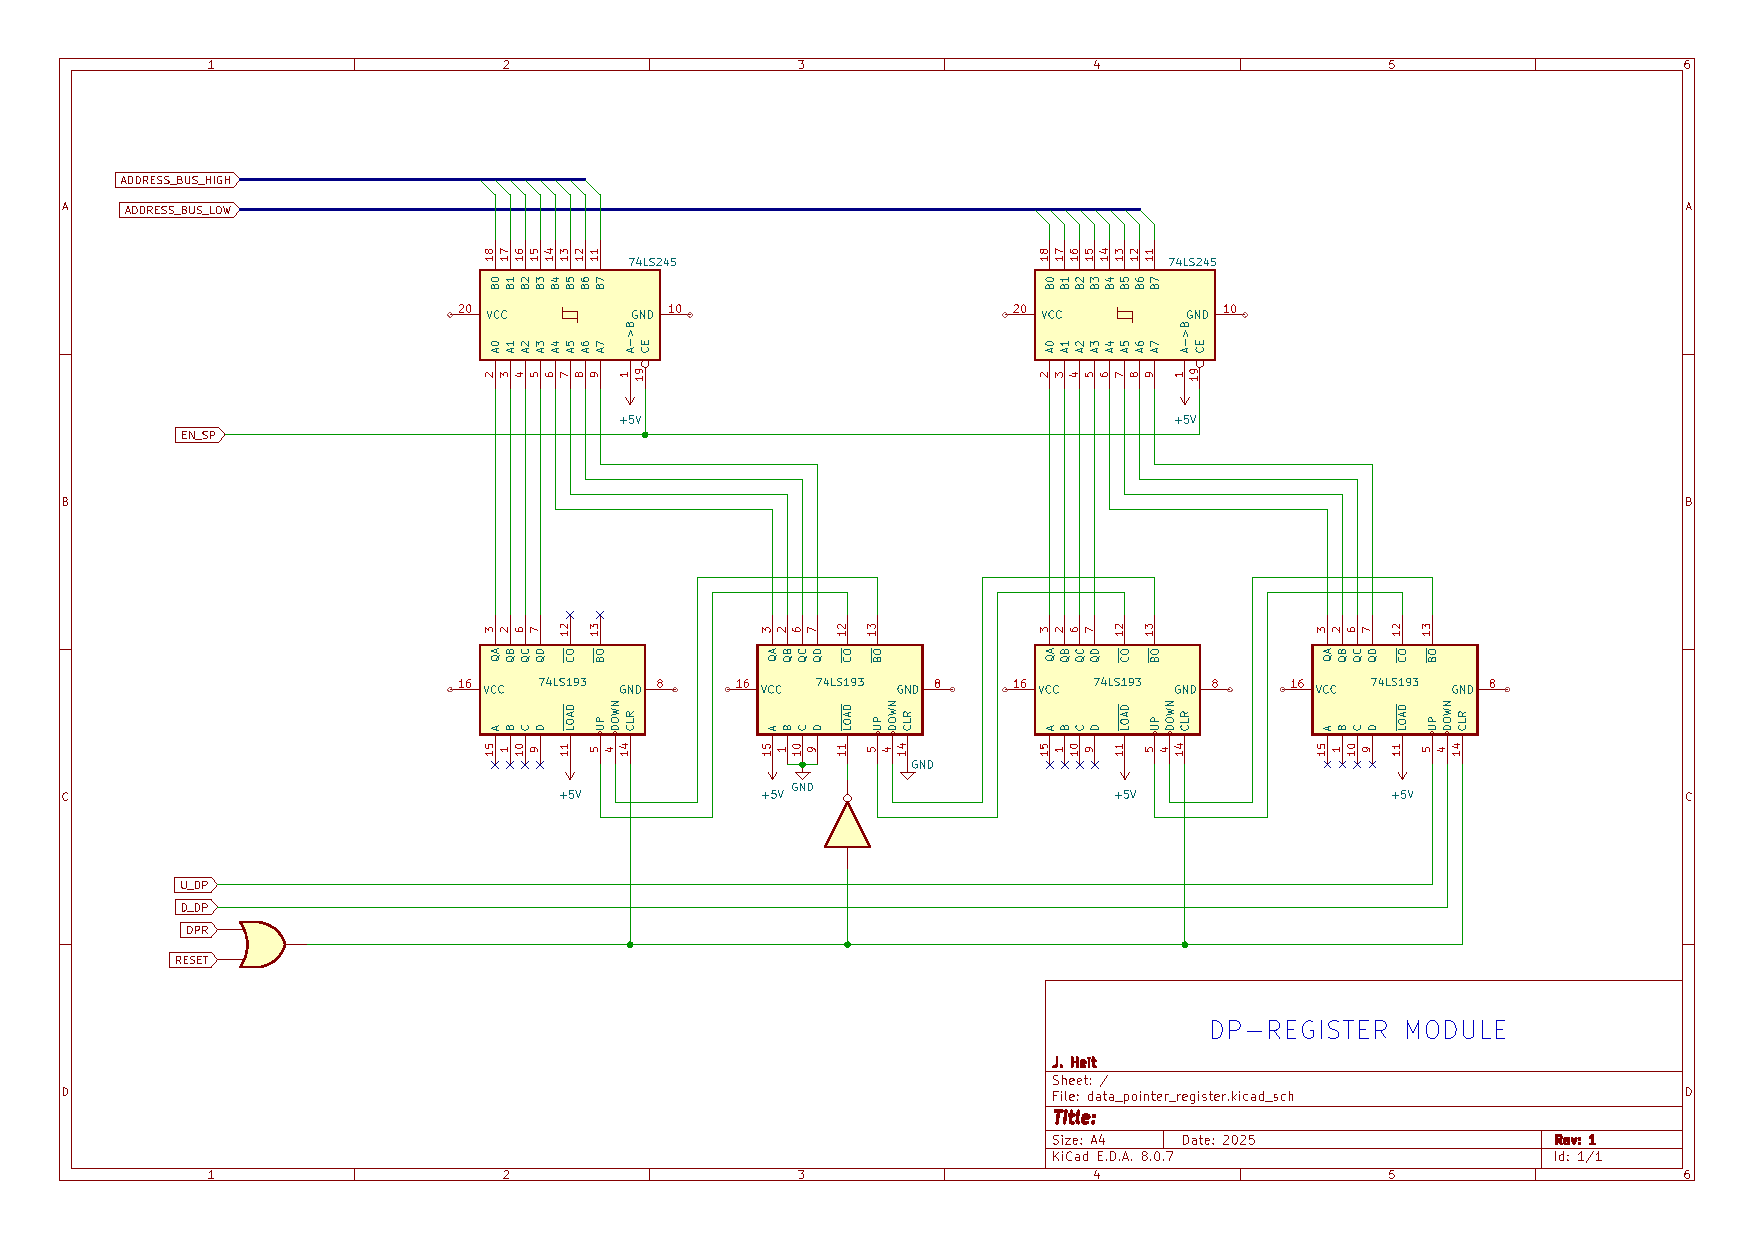
\includepdf[landscape=true]{schematics/datapointerregister.pdf}


%%%%%%% DATA REGISTER

\subsection{D Register Module}
\begin{figure}[H]
  % TODO: add annotations to the image
  \centering
  
\includegraphics[width=0.6\textwidth]{img/placeholder}
  \caption{Close up of the Data Register Module.}
  \label{fig:dregcloseup}
\end{figure}

The data register holds (a copy of) the value in memory currently pointed to by the datapointer. In the computer, it is located in the top left corner. It is based around the 74LS193 counting register and driven by the register driver described in Section \ref{sec:implementation:registerdriver}. The output is buffered in a tristate buffer (74LS245) before being connected to the databus. A second buffer is used to send all zeroes to the high byte of the databus since the data is only 8 bits wide. The buffers are set to output-mode only (even though the register is able to read from the bus as well) because the 74LS193 chips have seperate pins for incoming and outgoing data. The incoming data is read from the bus directly without going through a buffer.

This module also produces the Z flag, indicating that it is currently containing the value 0. This is achieved by sending the output through an array of OR gates and finally an inverter. The output is then sent to the second half of the instruction register which is responsible for keeping track of the flags.

Because the 74LS193 is loading asynchronously, the clock is gated together with the LD\_D signal through a NAND gate in order to load synchronously with the clock when the LD\_D signal is high (the load-pin on the '193 is active low). The necessity of a NAND gate meant it was easier to also implement any inverters needed in the circuit in terms of NAND gates.

\subsubsection*{Parts}
\begin{itemize}\itemsep0em
\item 1x 74LS00 (NAND)
\item 2x 74LS32 (OR)
\item 2x 74LS138 (3-to-8 demultiplexer)
\item 2x 74LS193 (Up/Down Counting Register)
\item 2x 74LS245 (Tristate Buffer)
\end{itemize}

\subsubsection*{Schematic}
A full schematic is provided on the next page.
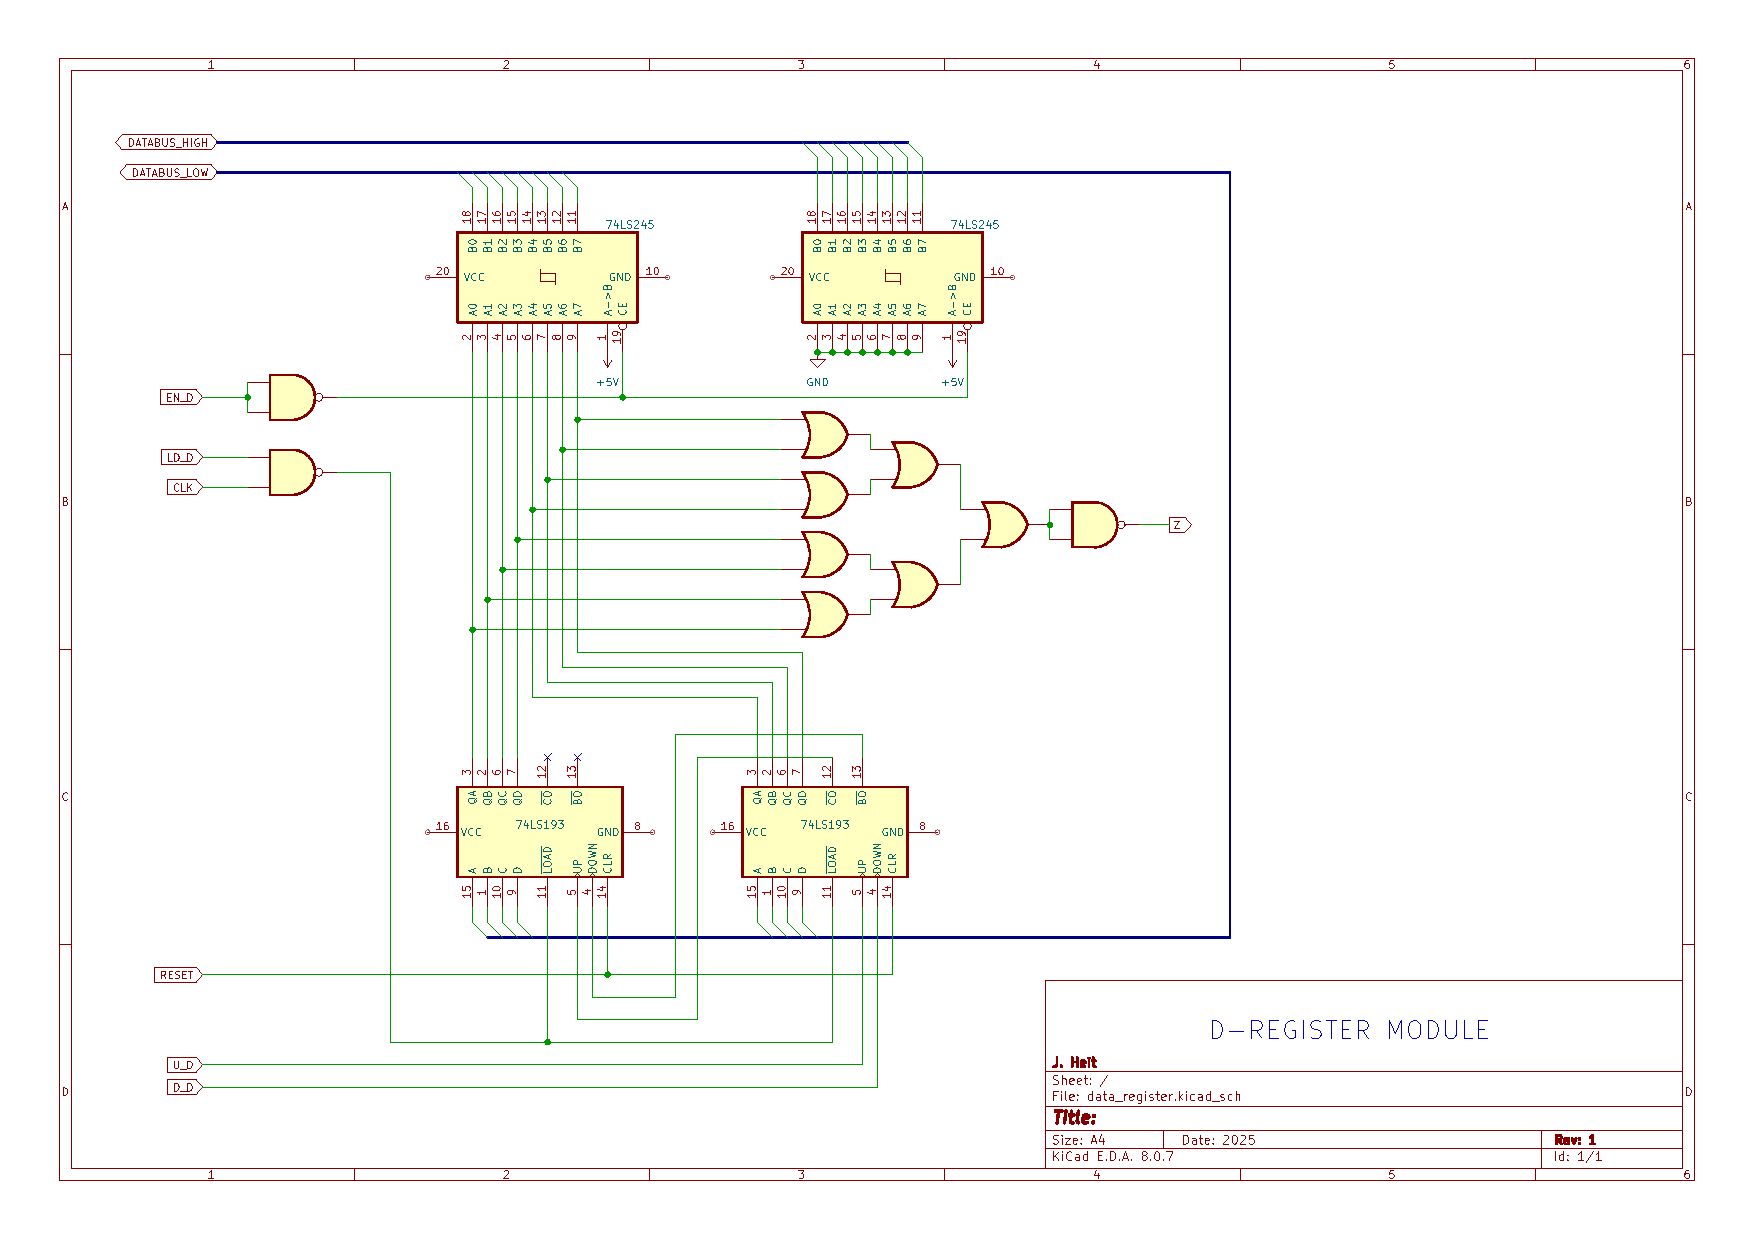
\includepdf[landscape=true]{schematics/dataregister.pdf}

%%%%%%% INSTRUCTION POINTER REGISTER

\subsection{IP Register Module}
\begin{figure}[H]
  \centering
  
\includegraphics[width=0.6\textwidth]{img/placeholder}
  \caption{Close up of the Instruction Register Module.}
  \label{fig:iregcloseup}
\end{figure}

The instruction pointer register holds a 16-bit value representing the address of an instruction in program-memory, stored in an EEPROM module (see \ref{sec:implementation:sigfetch}). Because the size of the available address space is $2^{14}$ instructions, the final two bits of the IP are not used. Red LEDs have been connected to these bits to quickly identify programs that try to address this non-existing part of program memory. The register IC's (74LS193) are driven by the register driver.

The IP is connected to the databus through two tristate buffers (74LS245) to avoid bus contention with the datapointer and keyboard module. It needs to be connected to this bus in order to write its value to the stack when a loop is entered. When exiting from a loop, a value is read back into the register through a direct connection to this bus (without going through a buffer). Because loading is done asynchronously on the '193, the load signal is NAND'ed with the clock to make loading synchronous again.

\subsubsection*{Parts}
\begin{itemize}\itemsep0em
\item 1x 74LS00 (NAND)
\item 4x 74LS193 (Up/Down Counting Register)
\item 2x 74LS245 (Tristate Buffer)
\end{itemize}

\subsubsection*{Schematic}
A full schematic is provided on the next page.
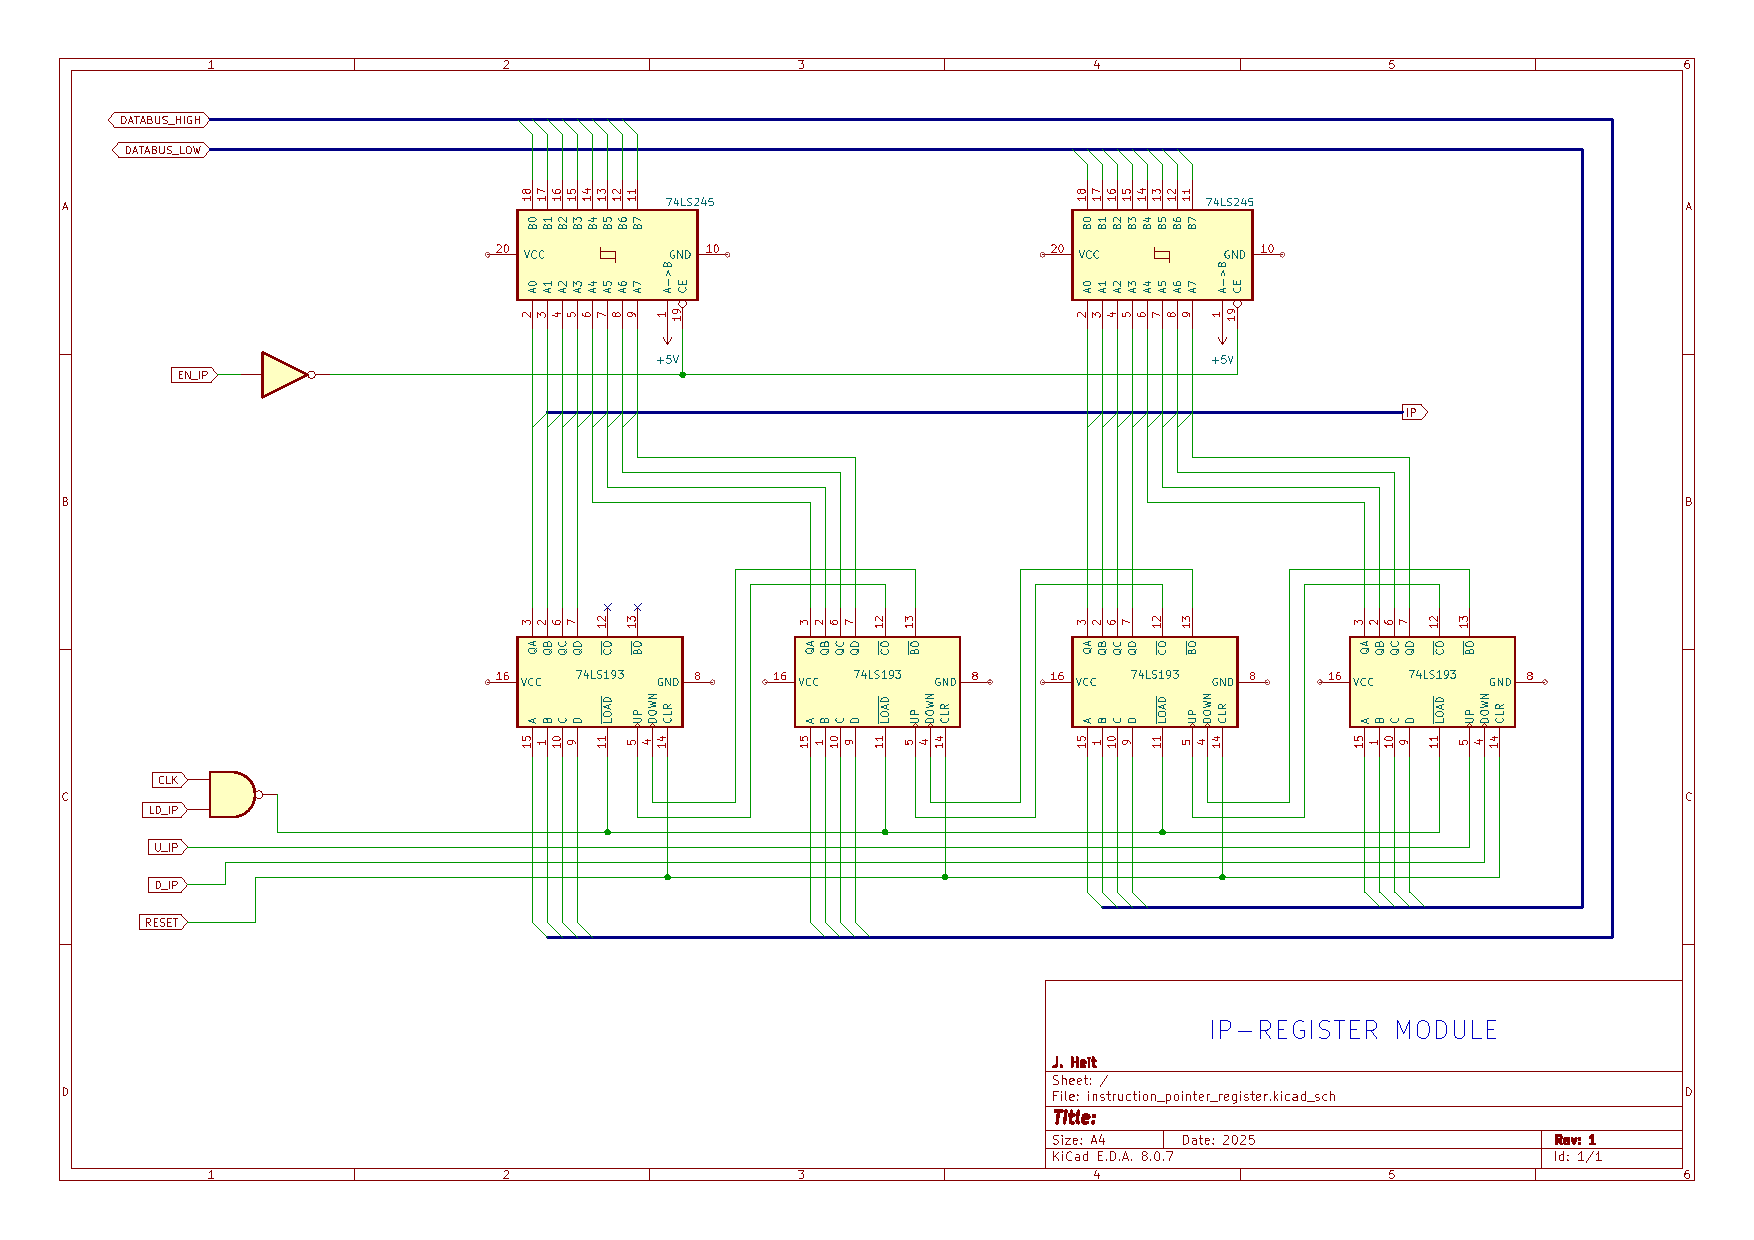
\includepdf[landscape=true]{schematics/instructionpointerregister.pdf}

%%%%%%% STACK POINTER REGISTER

\subsection{SP Register Module}
\begin{figure}[H]
  \centering
  
\includegraphics[width=0.6\textwidth]{img/placeholder}
  \caption{Close up of the Stack Pointer Register Module.}
  \label{fig:spregcloseup}
\end{figure}

The stack pointer is an 8 bit value representing a memory address in the range 0x00 - 0xff, which has been reserved to hold instruction pointer values. This is necessary for implementing conditional loops. When a loop is entered, the current value in the IP register is stored on the stack at the address pointed to by the stack pointer. The SP module is therefore connected to the same RAM address bus as the datapointer, which means it should go through a tristate buffer to avoid bus contention.

\subsubsection*{Parts}
\begin{itemize}\itemsep0em
\item 1x 74LS04 (NOT)
\item 2x 74LS193 (Up/Down Counting Register)
\item 2x 74LS245 (Tristate Buffer)
\end{itemize}

\subsubsection*{Schematic}
A full schematic is provided on the next page.
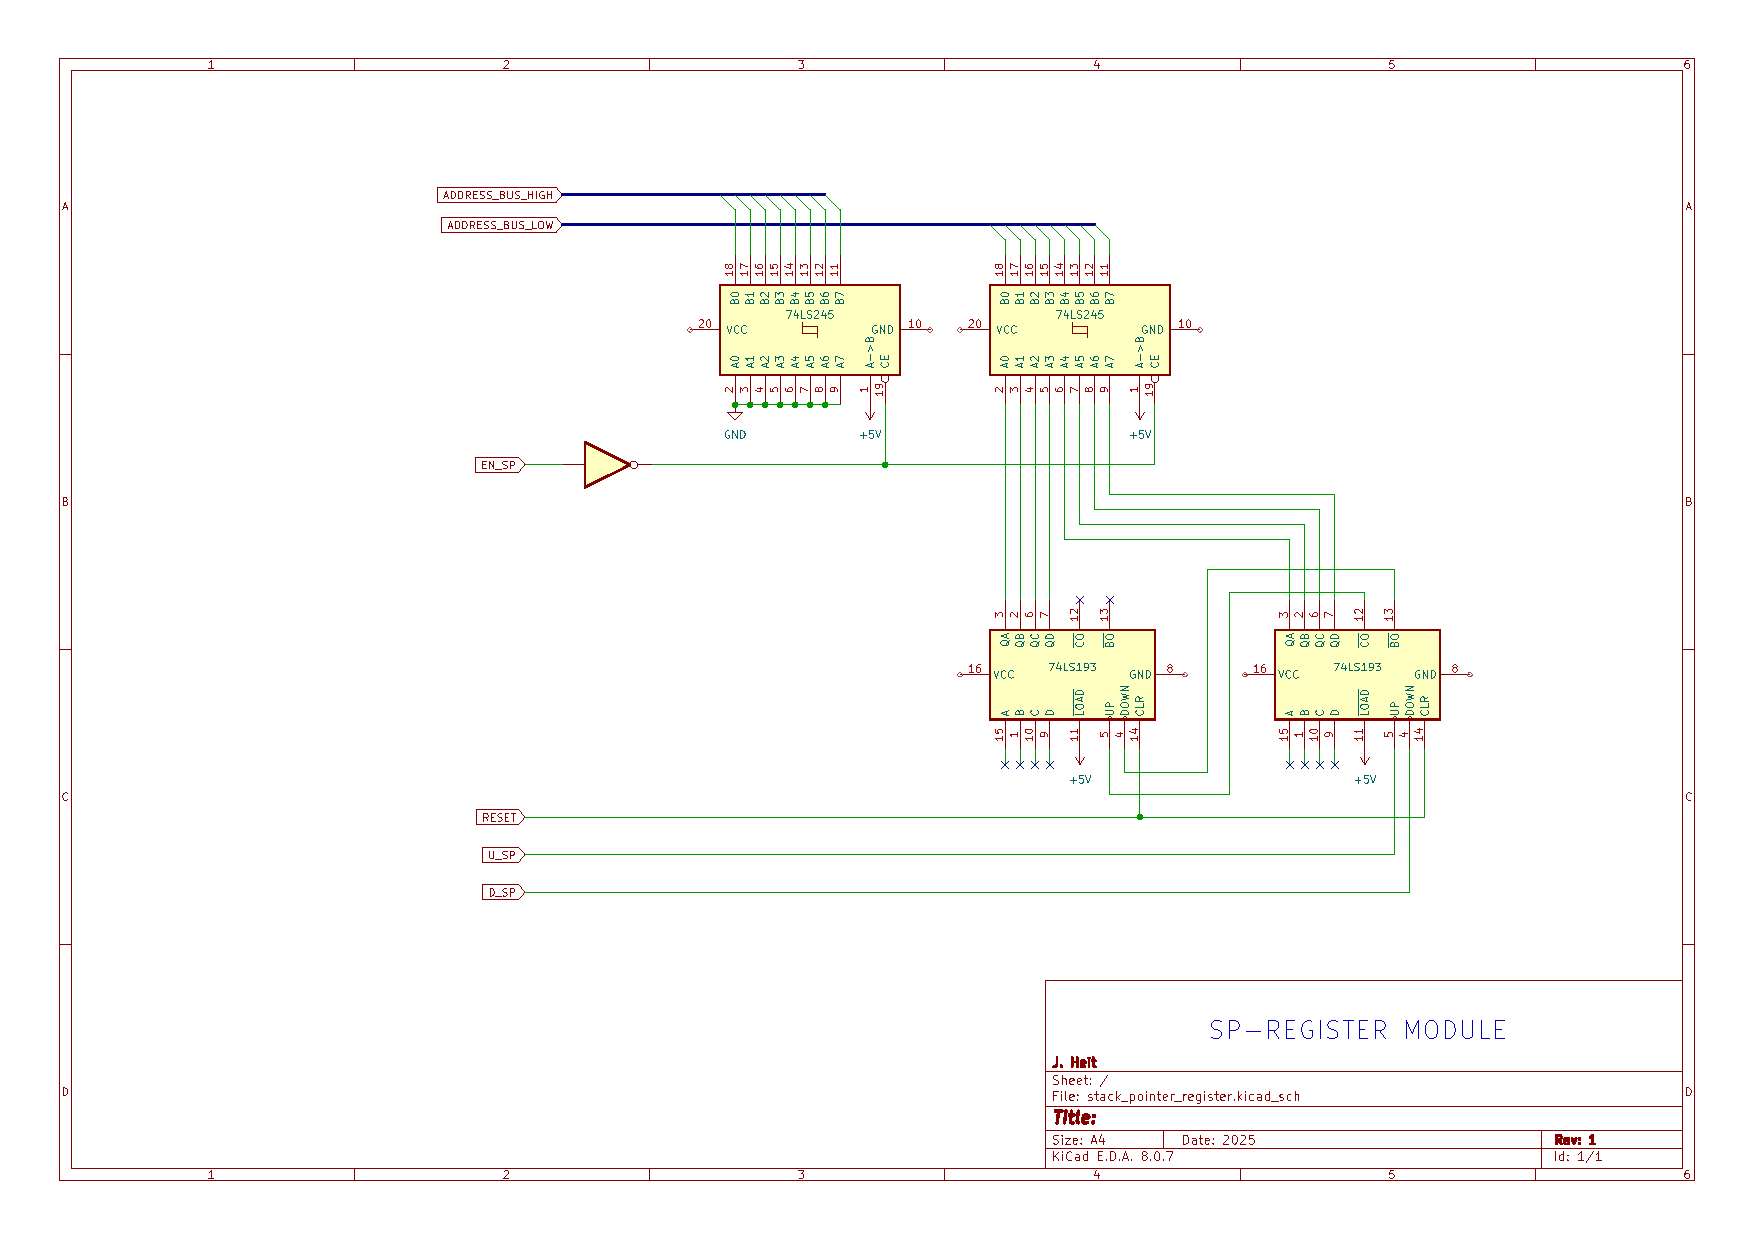
\includepdf[landscape=true]{schematics/stackpointerregister.pdf}


%%%%%%% CONTROL UNIT

\subsection{Control Unit}
\subsubsection{Partitioning}
The control unit is responsible for sending the appropriate signals to each of the modules. The general idea is that the current instruction pointed to by the IP (4 bits) together with the state flags (another 4 bits: A, V, S and Z) and the cycle count (3 bits) combine together to form an (11 bit) address into an EEPROM chip (AT28C64B) which contains the signal configuration for this state. The problem with this approach however is that the control unit needs to be able to drive 22 different control signals (for a complete list, see \ref{sec:architecture:cu}) or the schematic below), which cannot all be stored at a single 8-bit address in the EEPROM. There are two solutions to this problem:
\begin{enumerate}
\item Use 3 EEPROM chips, each containing a set of 8 signals (maximum). This allows for 24 different signals to be stored and retrieved efficiently in the same clock cycle.
\item Use 1 EEPROM chip and partition its memory space using its two unused address bits (the EEPROM has 13 address lines of which we so far needed only 11 to encode the state of the computer). In this case, additional logic and additional read-cycles are needed to gather the different parts of the control signal configuration.
\end{enumerate}

At the time of designing this processor, the AT28C64B was in very short supply and we were only able to find a single chip for use in the prototype. This forced us to implement method 2 at the cost of burning additional clock cycles to retrieve each of the three parts of the signal configuration. Even though this approach results in a significantly slower computer, it is an elegant solution in the sense that all of the microcode information is stored in a single place. It also somewhat simplified the testing process because we only had to reprogram a single EEPROM every time the microcode table turned out to contain an error, rather than 3 different chips (see \ref{sec:implementation:programmer} for details on how these chips are programmed).

Based on the physical layout of the board, the following configuration was used to partition the EEPROM:
\\
\begin{center}
\begin{tabular}{r|ll} 
  Address Bits & \\ \hline
  0-2  & Cycle count & ($000_2$ - $111_2$) \\
  3-4  & Partition number & ($00_2$ - $11_2$) \\
  5-8  & Instruction & ($0000_2$ - $1111_2$) \\
  9-12 & Flags & ($0000_2$ - $1111_2$) \\
\end{tabular}
\end{center}

\subsubsection{Clock Divider}
Due to the partitioning strategy, the master clock needs to be divided into 4 subclocks. On the first 3 subclock pulses, each of the control signal configuration parts is loaded into an 8-bit partition register, connecting to the modules that expect the corresponding signals. A pulse from the fourth subclock is then sent to all of the modules to execute their functions. 

To implement the clock divider, a single 4-bit counting register (74LS161) is connected to address bits 3 and 4 of the EEPROM and to demultiplexer (74LS138). The first 3 outputs of the demultiplexer produce the first 3 subcycle pulses which are sent to 3 sets of two 4-bit registers (also 74LS161 with counting disabled), which will store each of the configuration parts. A '161 will load the value at its input reliably when the load-pin is active before receiving a pulse from the clock. This is why the outputs of the '138 are directly connected to the load-pins but also negated and AND'ed with the clock to produce a pulse offset by a half-cycle on the clock pins of the '161s (Figure \ref{fig:partitioning}). The fourth output of the demux is used as the clock signal for all the other modules (CLK) and to reset the count of the '161 that is responsible for keeping track of the partition numbers to make it loop back to 0, restarting the process for the next instruction.

\begin{figure}[H]
  \centering
  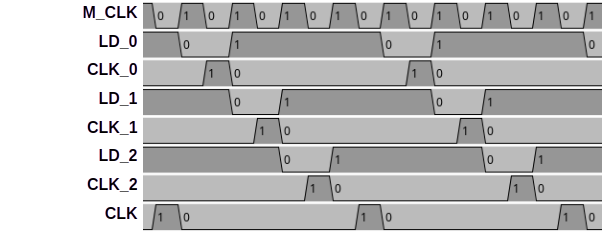
\includegraphics[width=0.8\textwidth]{img/partitioning}
  \caption{Timing diagram of the signals going from the clock divider to the load and clock pins of the partition registers (load pins are active low on the 74LS161).}
  \label{fig:partitioning}
\end{figure}

\subsubsection{Program ROM}
The actual BF program is stored in another 8K EEPROM chip (AT28C64) and is addressed by the instruction pointer as mentioned before. Since each BF instruction only needs 4 bits to be encoded (there are less than 16 different instructions), we can store up to 16K instruction in the chip by packing 2 consecutive instructions together in a single byte (handled by the assembler). Rather than using bit 0 from the IP directly as address bit 0 on the EEPROM, it is used as the data-select signal to a 74LS157 multiplexer. This multiplexer takes 1 select-bit and two sets of 4 databits. Depending on the value of the select-bit, one of the sets of 4-bit data is sent to its outputs. This allowes us to select either the low or high nibble of the data in the EEPROM, effectively doubling the amount of instructions that can be stored and retrieved.

\subsubsection{Instruction and Flag Register}
The instruction register acts as a buffer to store the current state of the system (current instruction + flags). It is connected to the output of the '157 described above, to the S and Z flags produced by the D and LS registers, and finally to the outputs of the flag register. The flag register gets its inputs directly from the control signals in order to buffer the A and V flag, which may be set at any cycle of an instruction and must be remembered until the next instruction (only 2 of its 4 bits are used).
